\documentclass[main.tex]{subfiles}
\begin{document}
\chapter{Introduction}
Why this data set?
Why deep learning?
What is the context?

\section{Medical Context}
In Germany 34.490 men and 18.030 women were diagnosed with an illness corresponding to the ICD-10 code C33-34 in 2012 \cite{koch2015krebs}. This code describes malignant tumors in the breathable tract more generally summarized as lung cancer. 43499 people died from this illness, which makes it one of the most dangerous types of cancer in Germany. The international comparison shows that other countries too suffer under it's impact.

\begin{figure}[h]
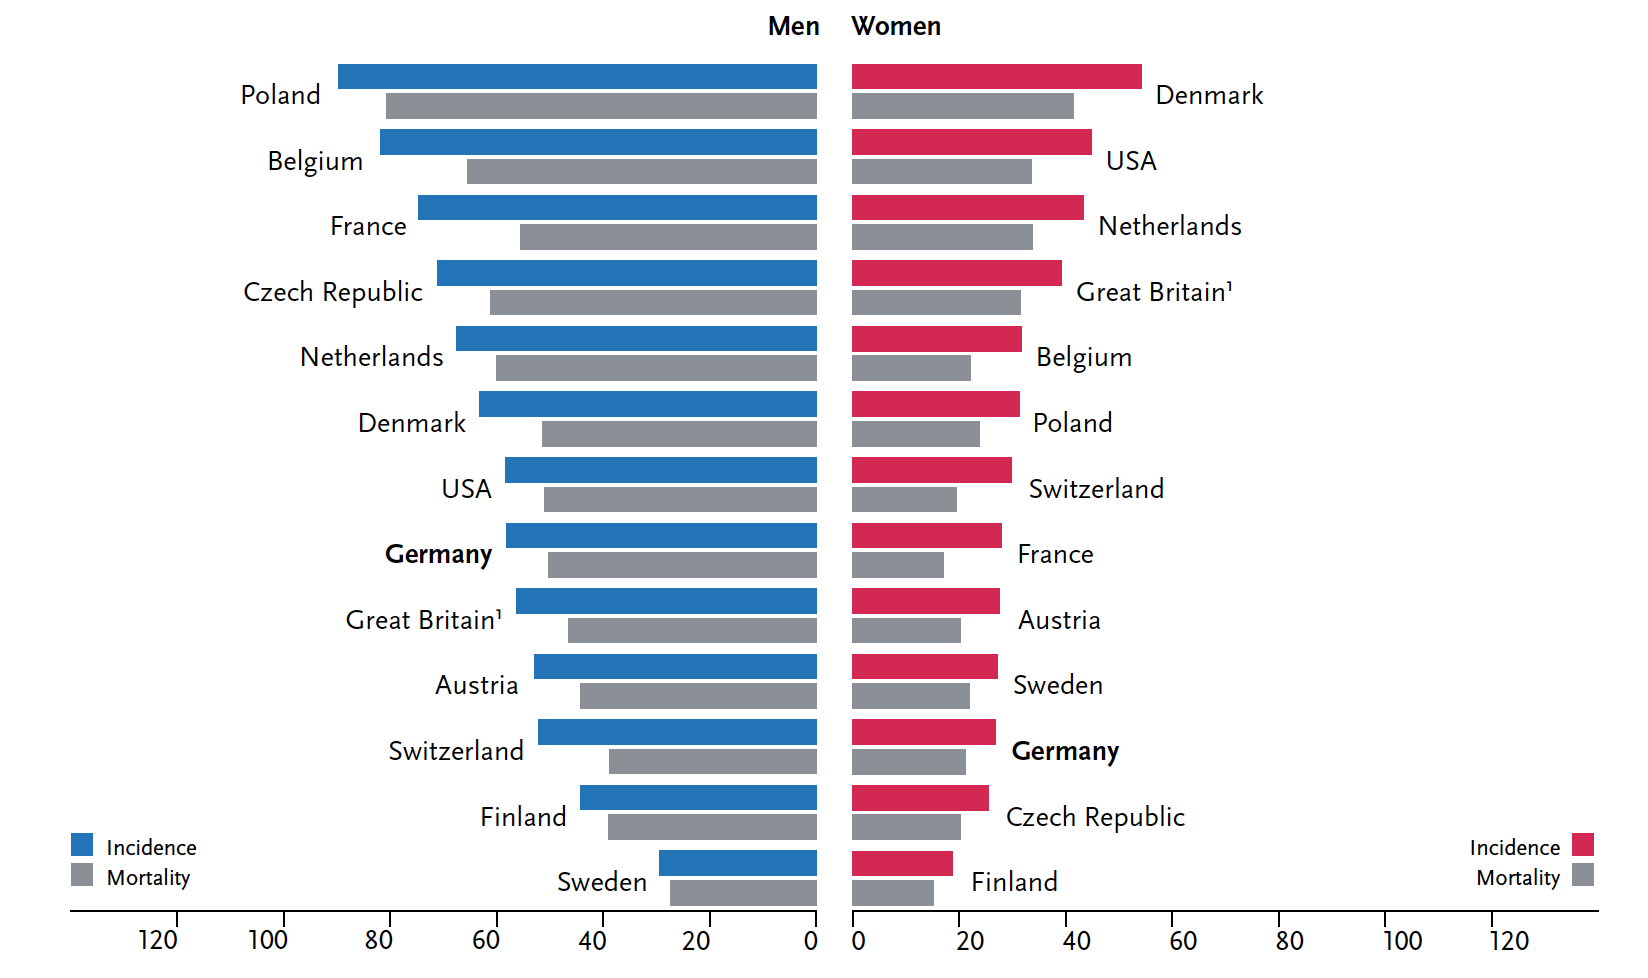
\includegraphics[width=\textwidth]{cancerInternational.png}
\caption{International comparison of age-standardized and mortality rates for lung cancer in the year 2012}
\end{figure}

The main risk factor has been shown to be the exposure to tobacco smoke, whether it's active consumption via cigarettes, or passive exposure especially in closed rooms. CT scanners are used to detect irregular tissue in a patients lung region. I

\section{Overview}


 A pulmonary nodule is a small, round (parenchymal nodule) or worm (juxtapleural nodule) shaped lesion in the lungs
 ground glass opacity nodules.
 
 GGO nodules are more likely to be malignant than solid nodules
There exist many algorithmic approaches to finding nodules in CT-Scans \cite{papers_classical} and some that
make use of deep convolutional neural networks to solve this task \cite{papers_dnn}

\section{Current Medical Approach}
Requirement to analyse X pictures per patient
current programs (screenshot OsiriX)
fallacy rates

\section{Opportunities for Assistance}

Early detection of lung cancer is important, because it avoids unnecessary scans in the scenario
of undetected cancerous material and it improves the error rate of radiologists.

Despite much effort being devoted to the computer-aided nodule detection problem, lung CAD systems remain an ongoing
research topic [18]. One of the major difficulties is the detection of GGO nodules with low-dose thin-slice CT screening. Another two difficulties are the detection of nodules that are adjacent to vessels or the chest wall when they have very similar intensity; and the detection of nodules that are nonspherical in shape. In such cases, intensity thresholding or model-based methods might fail to identify those nodules.

\section{Gaining insights from Deep Neural Networks}
Neural networks are strong tools that recently have been shown to solve all kind of problems. They can play
computer games and drive a car, they can create new art and play go to name only a few examples. Yet it seems like the solution they come up with is not intelligible to humans. But in a scenario where medical decisions are based on the output of an algorithm it is crucial that the algorithm is reliable and the way it comes up with a decision is accepted by the people responsible. As long as this is not the case it might still happen that the network produces erroneous results in some cases that did not occur during training.

Strategies to cope with this problem include:
\begin{itemize}
\item huge databases that contain a variety of samples. In this thesis an open dataset is used that was
the result of a cooperative effort of many scientists and medical staff members and has proven
it's worth in many publications. A possible downside is still that the patients in this database are all Americans

\item leaving the final decision up to a specialist. Makes sense in any case. But as the expert relies more and more on the assisting systems, hidden biases can influence the specialists decision - meaning that their combined performance might diminish over time.
\end{itemize}


But at the end of the day a neural network only stays to be a tool as long as no further insights into
the problem can be gained through it's solution. This is why this thesis is concerned with extracting
features and and solution mechanisms from a trained deep neural network on the example of lung CT data.

\end{document}
